\documentclass{beamer}
\usepackage{beamerthemeshadow}
\usepackage{algpseudocode}
\usepackage{listings}
\usepackage{color}
\usepackage{setspace}
\usepackage{array}
\usepackage[USenglish]{babel}
\usepackage[useregional]{datetime2}



\DTMlangsetup[en-US]{showdayofmonth=false}

\definecolor{Code}{rgb}{0,0,0}
\definecolor{Decorators}{rgb}{0.5,0.5,0.5}
\definecolor{Numbers}{rgb}{0.5,0,0}
\definecolor{MatchingBrackets}{rgb}{0.25,0.5,0.5}
\definecolor{Keywords}{rgb}{0,0,1}
\definecolor{self}{rgb}{0,0,0}
\definecolor{Strings}{rgb}{0,0.63,0}
\definecolor{Comments}{rgb}{0,0.63,1}
\definecolor{Backquotes}{rgb}{0,0,0}
\definecolor{Classname}{rgb}{0,0,0}
\definecolor{FunctionName}{rgb}{0,0,0}
\definecolor{Operators}{rgb}{0,0,0}
\definecolor{Background}{rgb}{0.98,0.98,0.98}

% Tables
\newcolumntype{L}[1]{>{\raggedright\let\newline\\\arraybackslash\hspace{0pt}}m{#1}}
\newcolumntype{C}[1]{>{\centering\let\newline\\\arraybackslash\hspace{0pt}}m{#1}}
\newcolumntype{R}[1]{>{\raggedleft\let\newline\\\arraybackslash\hspace{0pt}}m{#1}}

\lstset{
    language=Python,
    literate={á}{{\'a}}1
        {ã}{{\~a}}1
        {é}{{\'e}}1
        {ó}{{\'o}}1
        {í}{{\'i}}1
        {ñ}{{\~n}}1
        {¡}{{!`}}1
        {¿}{{?`}}1
        {ú}{{\'u}}1
        {Í}{{\'I}}1
        {Ó}{{\'O}}1
}

% Language 
\lstdefinelanguage{Python}{
numbers=left,
numberstyle=\footnotesize,
numbersep=1em,
xleftmargin=1em,
framextopmargin=2em,
framexbottommargin=2em,
showspaces=false,
showtabs=false,
showstringspaces=false,
frame=l,
tabsize=4,
% Basic
basicstyle=\ttfamily\small\setstretch{1},
backgroundcolor=\color{Background},
% Comments
commentstyle=\color{Comments}\slshape,
% Strings
stringstyle=\color{Strings},
morecomment=[s][\color{Strings}]{"""}{"""},
morecomment=[s][\color{Strings}]{'''}{'''},
% keywords
morekeywords={import,from,class,def,for,while,if,is,in,elif,else,not,and,or,print,break,continue,return,True,False,None,access,as,,del,except,exec,finally,global,import,lambda,pass,print,raise,try,assert},
keywordstyle={\color{Keywords}\bfseries},
% additional keywords
morekeywords={[2]@invariant,pylab,numpy,np,scipy},
keywordstyle={[2]\color{Decorators}\slshape},
emph={self},
emphstyle={\color{self}\slshape},
%
}

\title[Introducci\'on a Big Data] %optional
{ Introducci\'on a Big Data }
 
\subtitle{Taller}
 
\author[JGM] % (optional, for multiple authors)
{Ing.~Gómez~Marín,~Jaime}
 
\institute[TECSUP] % (optional)
{
  
    Departamento de TdG
}
 
\date{\today} 

\logo{\centering 
\includegraphics[height=0.8cm]{img/tecsup.png}}

\begin{document}
\begin{frame}
\titlepage
\end{frame}

% Index
\begin{frame}
\frametitle{\'Indice}
\begin{itemize}
\item ¿Qu\'e es Big Data?
\item Mas allá del Hype
\item Big Data y la Ciencia de Datos
\item Procesando el Big Data
\item Bibliograf\'ia
\end{itemize}
\end{frame}

% Introduccion
\begin{frame}
\frametitle{Introducci\'on}
 
En esta sesi\'on se aprender\'a a usar  estructura de datos con los siguiente tipos de datos : 
\alert{Tupla}, \alert{List} , \alert{Set} y \alert{Dictionary} en Python.

\end{frame}

% Big Data y la Ciencia de Datos
\begin{frame}
\frametitle{Aspectos de una plataforma de Big Data }

\begin{itemize}
\item Integraci\'on 
\item Analisis
\item Visualizaci\'on
\item Optimizaci\'on
\item Securidad
\item Gobernanza
\end{itemize}

\end{frame}

\begin{frame}
\frametitle{Escalas de los datos}
\begin{figure}
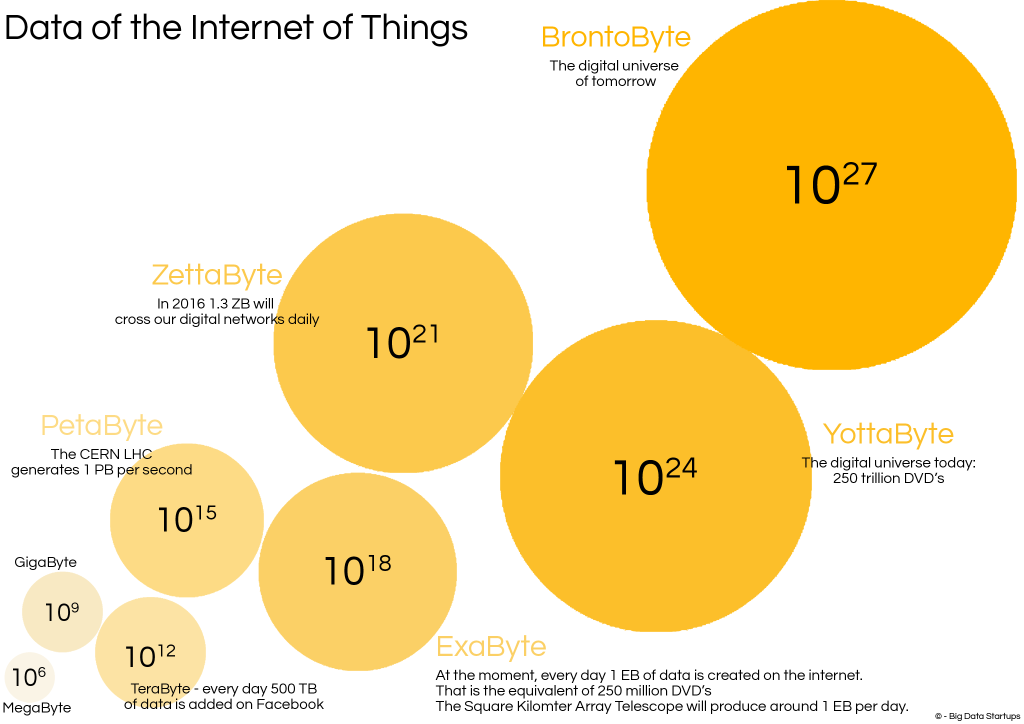
\includegraphics[scale=0.26]{img/2_Hyper}
\end{figure}
\end{frame}

\begin{frame}
\frametitle{Cloud Computing}
\begin{figure}
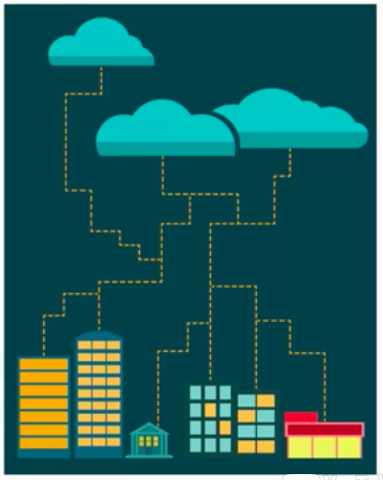
\includegraphics[scale=0.35]{img/2_CloudComputing}
\end{figure}
\end{frame}

\begin{frame}
\frametitle{¿De donde viene los datos?}
Las 3 mayores fuentes de datos: \\
\begin{itemize}
\item Datos generados por las personas
\item Datos generados por las m\'aquinas
\item Datos generados por los negocios
\end{itemize}
\end{frame}


\begin{frame}
\frametitle{¿Qu\'e es Big Data?}
\begin{figure}
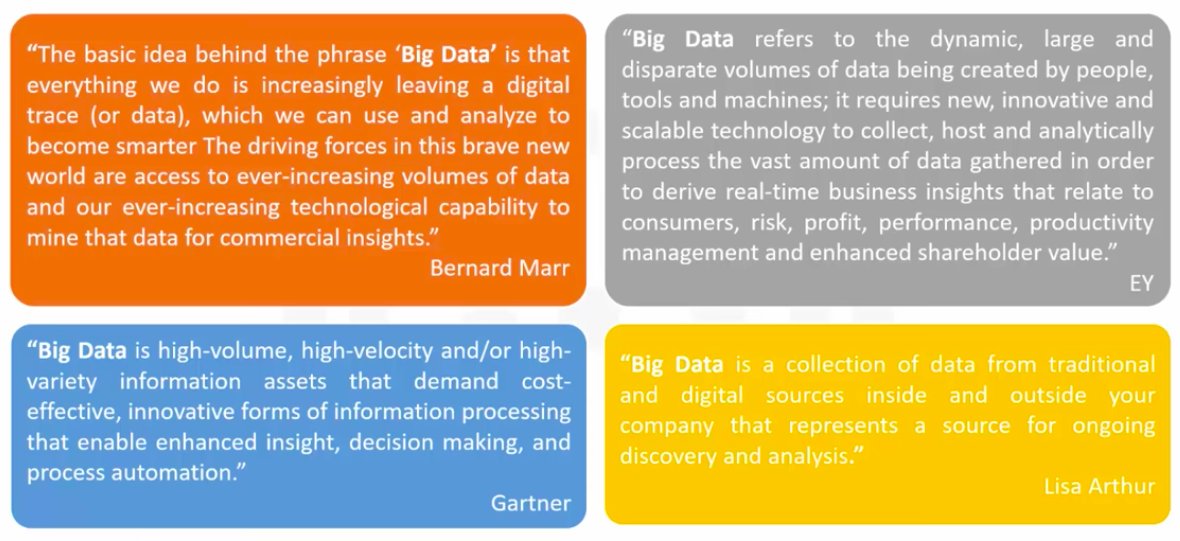
\includegraphics[scale=0.18]{img/1_BigData_Definition}
\end{figure}
\end{frame}

\begin{frame}
\frametitle{Las 5 V de Big Data}
\begin{figure}
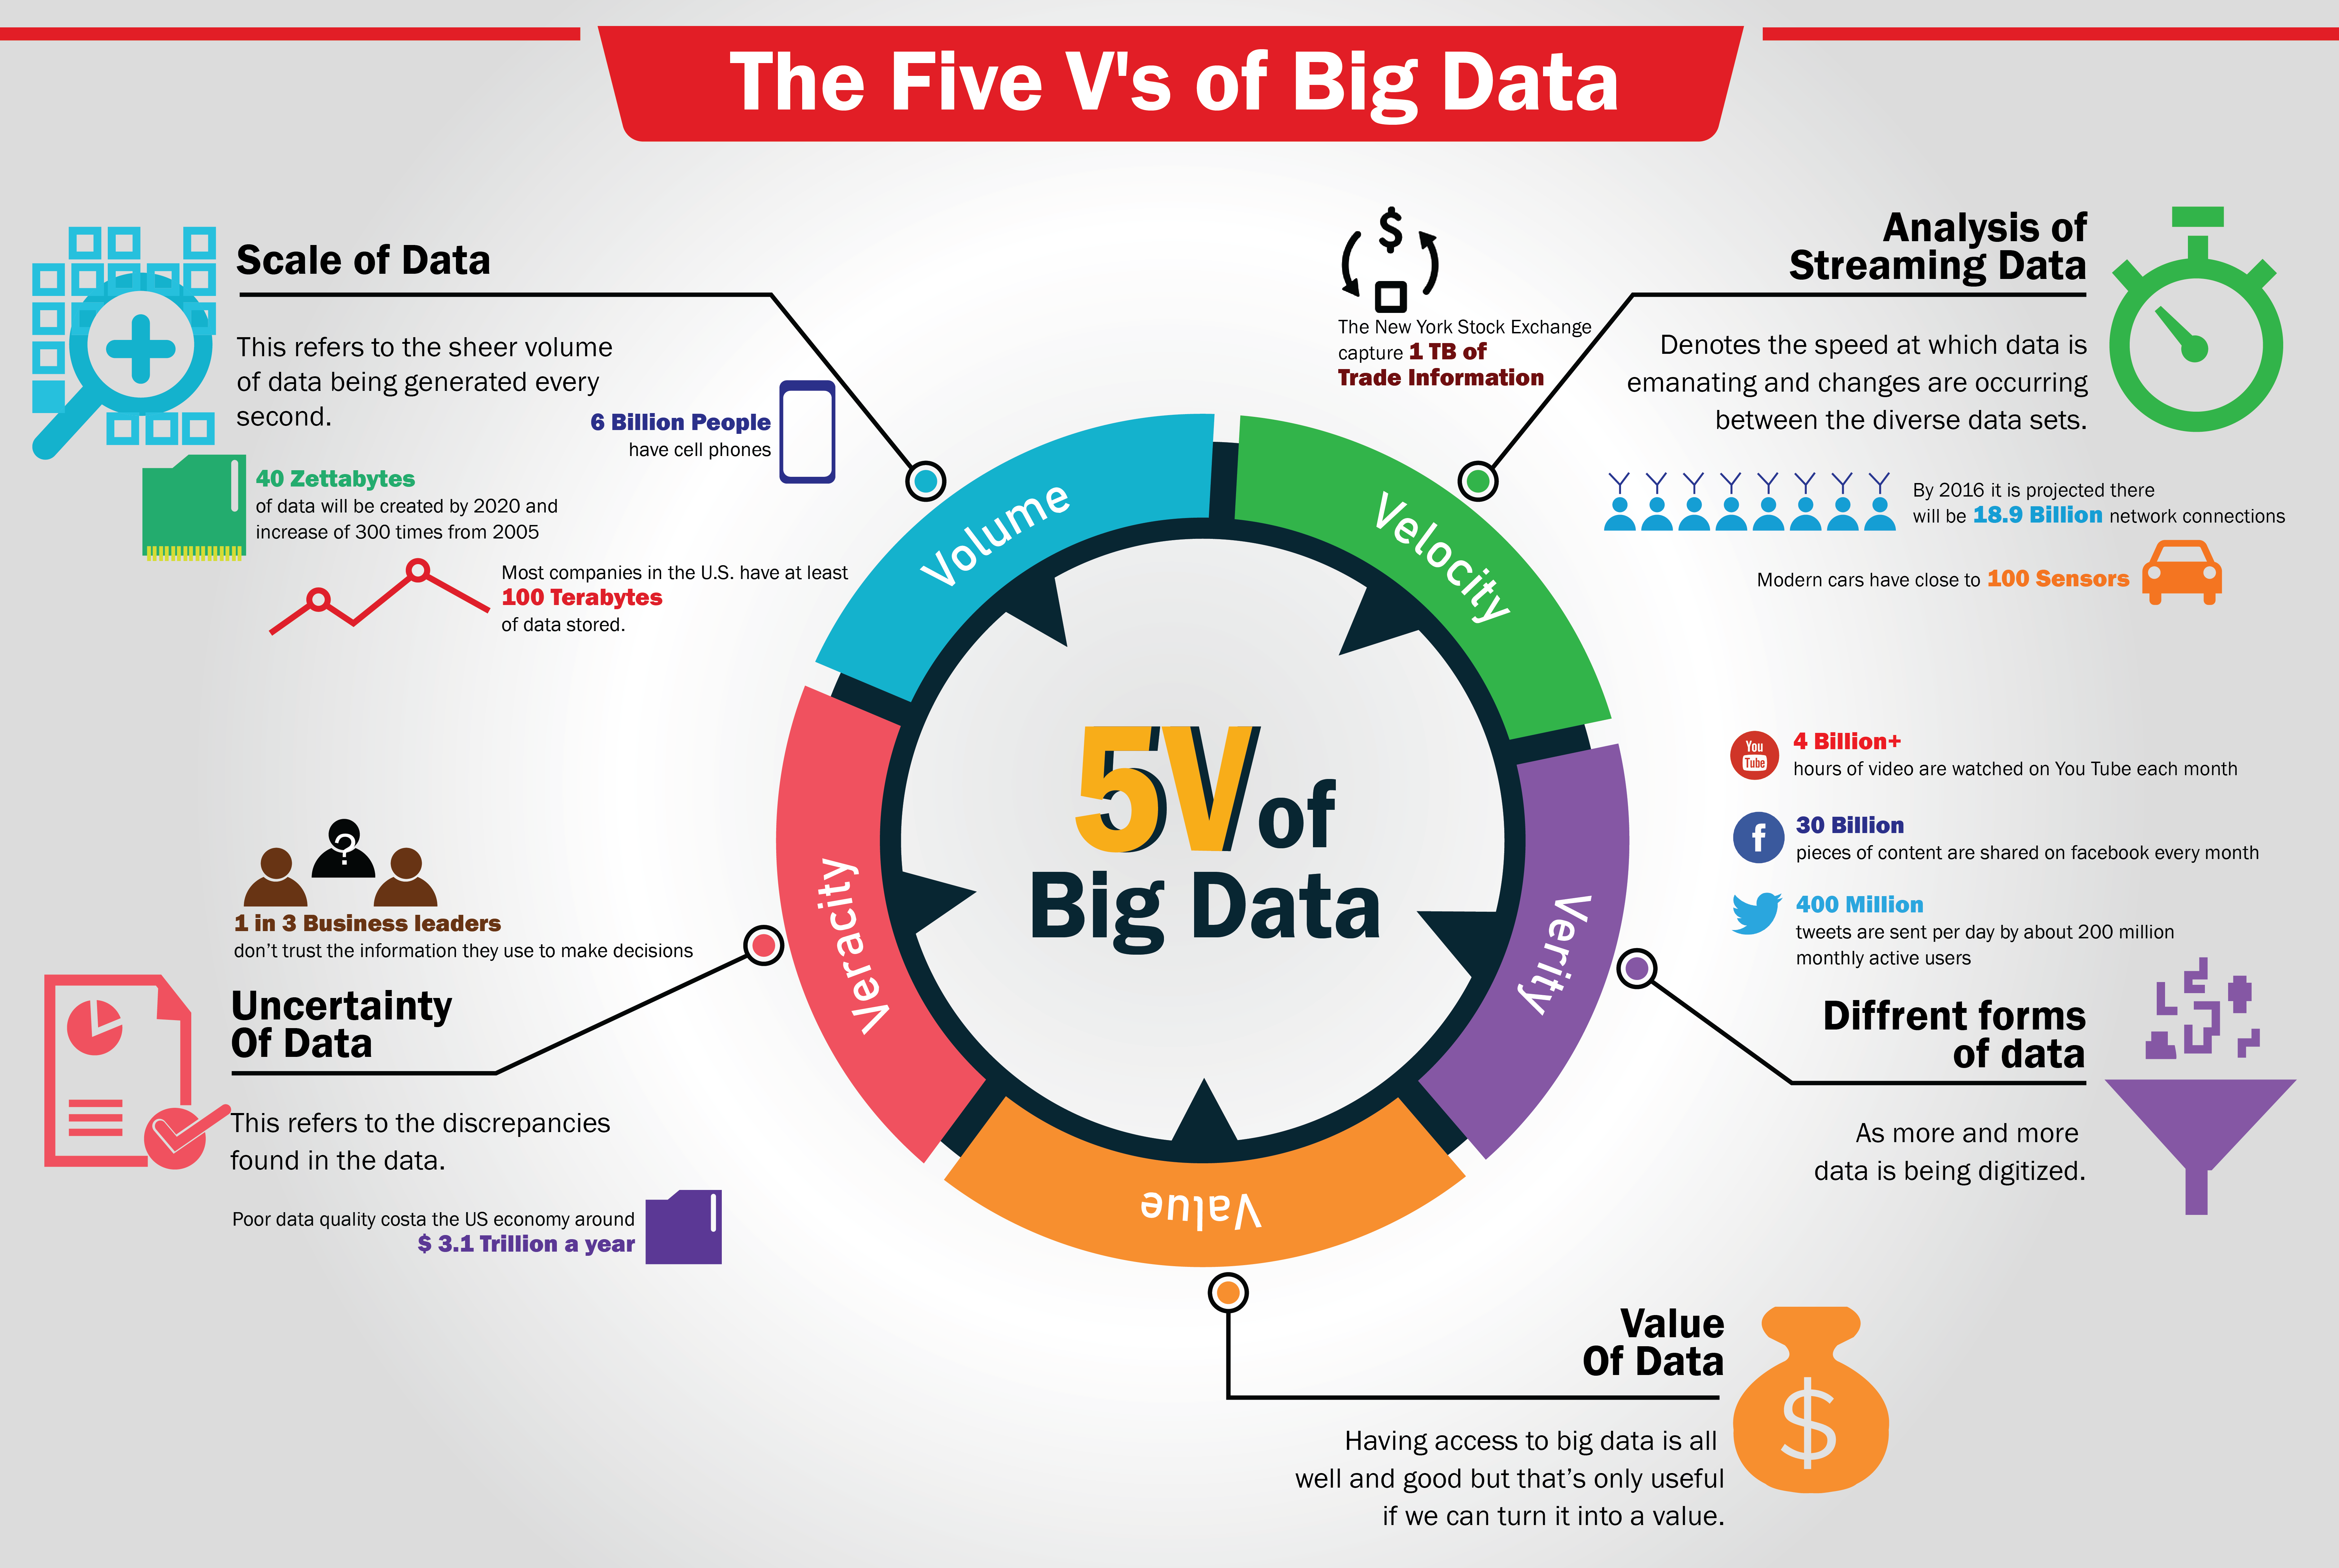
\includegraphics[scale=0.18]{img/1_BigData_5V}
\end{figure}
\end{frame}



\begin{frame}
\frametitle{Big Data Skills}
Descubrir y analizar las tendencias que ocurren en los datos
\begin{figure}
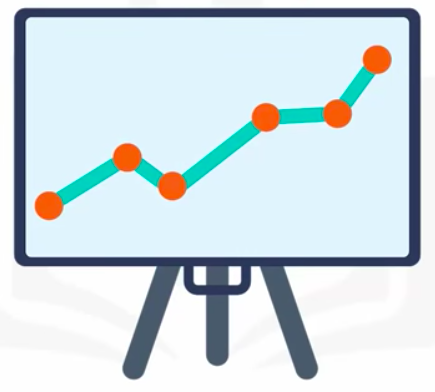
\includegraphics[scale=0.3]{img/2_BigData_Skill}
\end{figure}
\end{frame}

\begin{frame}
\frametitle{Big Data : Fuentes}
\begin{figure}
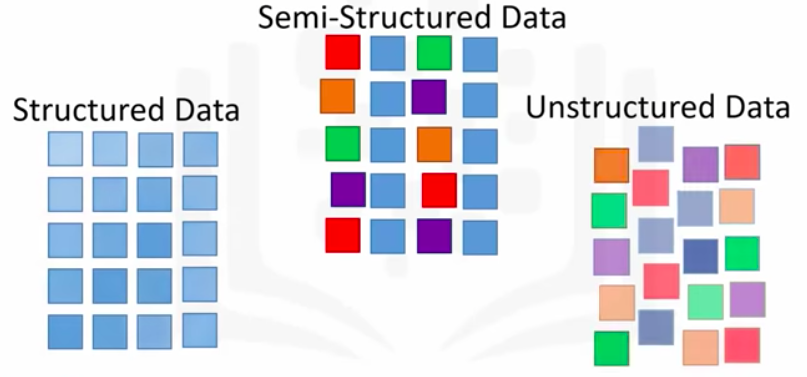
\includegraphics[scale=0.3]{img/2_BigData_DataSources}
\end{figure}
\end{frame}


\begin{frame}
\frametitle{Structured Data}
\begin{figure}
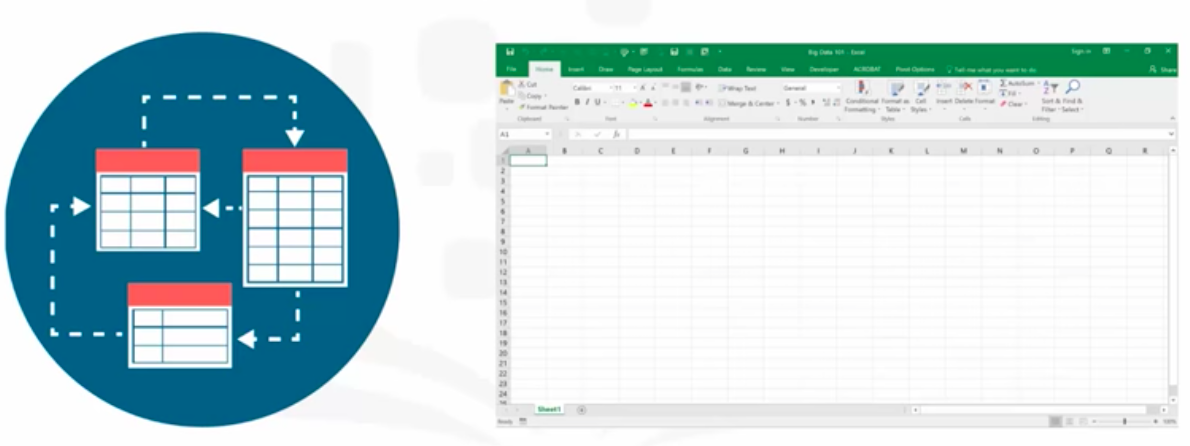
\includegraphics[scale=0.25]{img/2_Structured_Data}
\end{figure}
\end{frame}

\begin{frame}
\frametitle{Semi Structured Data}
\begin{figure}

\includegraphics[scale=0.25]{img/2_Semi_Structured_Data}
\end{figure}
\end{frame}


\begin{frame}
\frametitle{Unstructured Data}
\begin{figure}
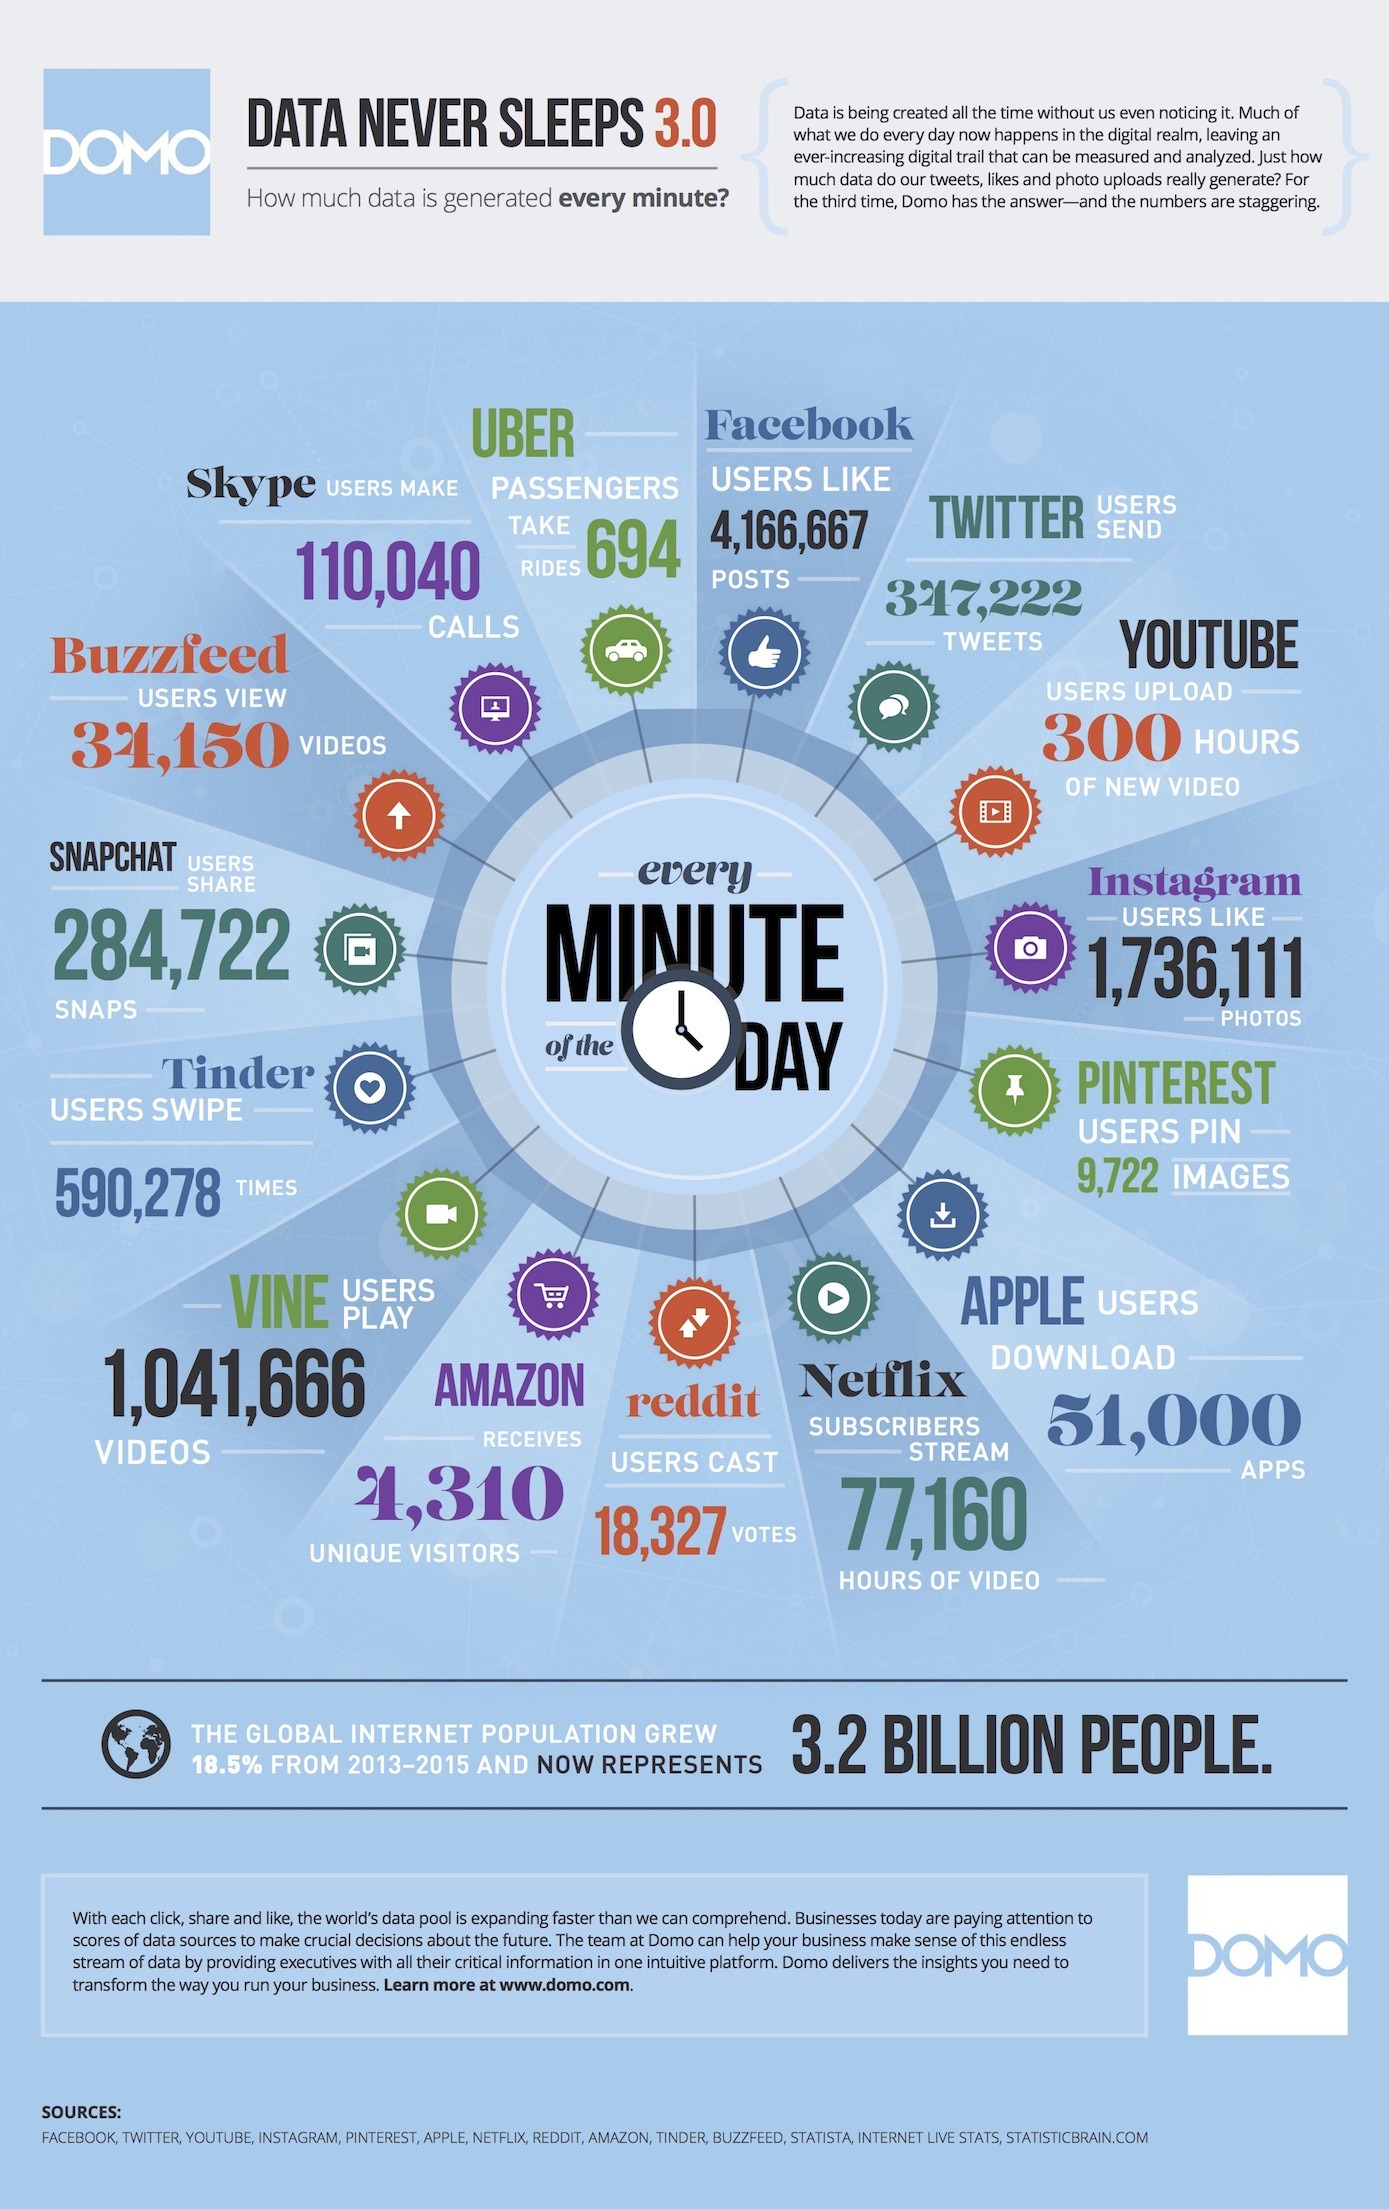
\includegraphics[scale=0.11]{img/2_Unstructured_Data}
\end{figure}
\end{frame}



\begin{frame}
\frametitle{Aspectos de una plataforma de Big Data : Integraci\'on}
\begin{figure}
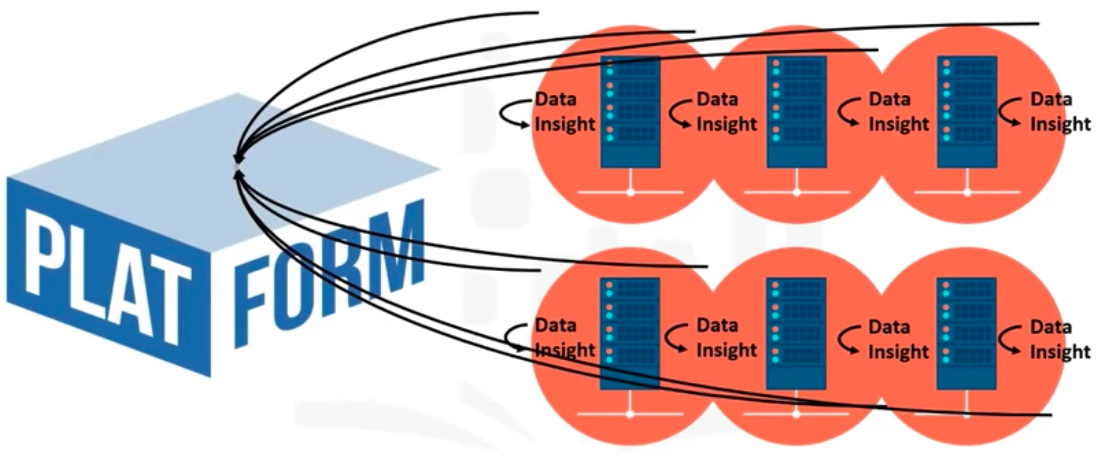
\includegraphics[scale=0.3]{img/3_Integration}
\end{figure}
\end{frame}

\begin{frame}
\frametitle{Aspectos de una plataforma de Big Data : An\'alisis}
\begin{figure}
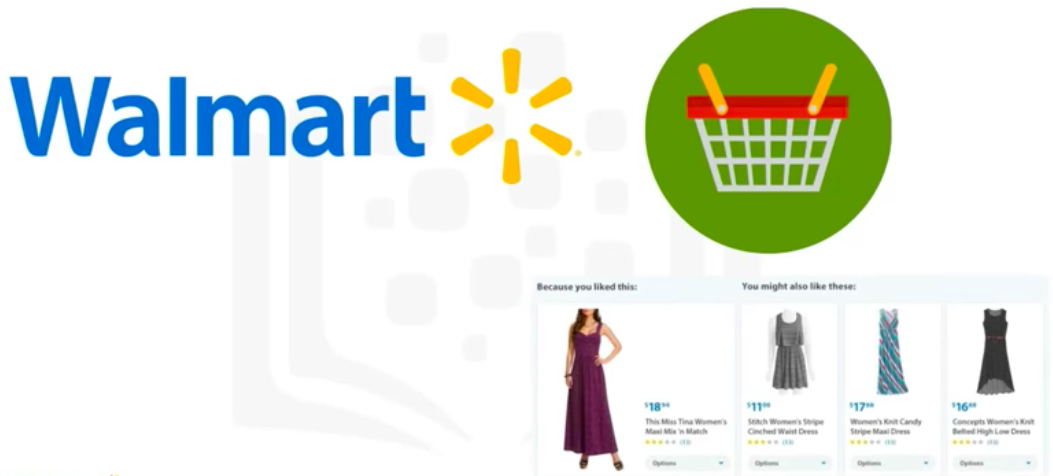
\includegraphics[scale=0.3]{img/3_Analysis}
\end{figure}
\end{frame}

\begin{frame}
\frametitle{Aspectos de una plataforma de Big Data: Visualizaci\'on}
\begin{figure}
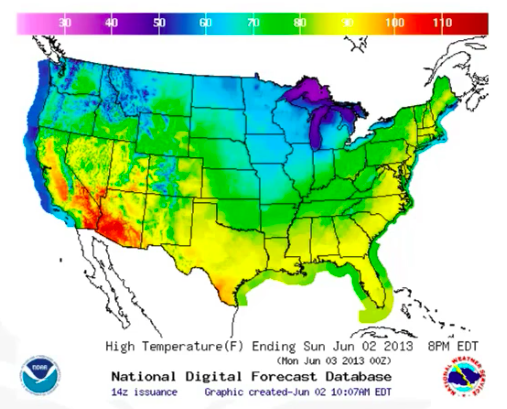
\includegraphics[scale=0.4]{img/3_Visualization}
\end{figure}
\end{frame}

\begin{frame}
\frametitle{Aspectos de una plataforma de Big Data : Seguridad}
\begin{figure}
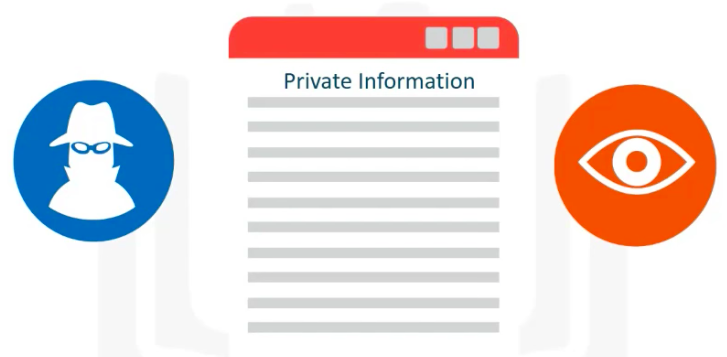
\includegraphics[scale=0.35]{img/3_Security}
\end{figure}
\end{frame}

\begin{frame}
\frametitle{Aspectos de una plataforma de Big Data : Gobernanza}
\begin{figure}
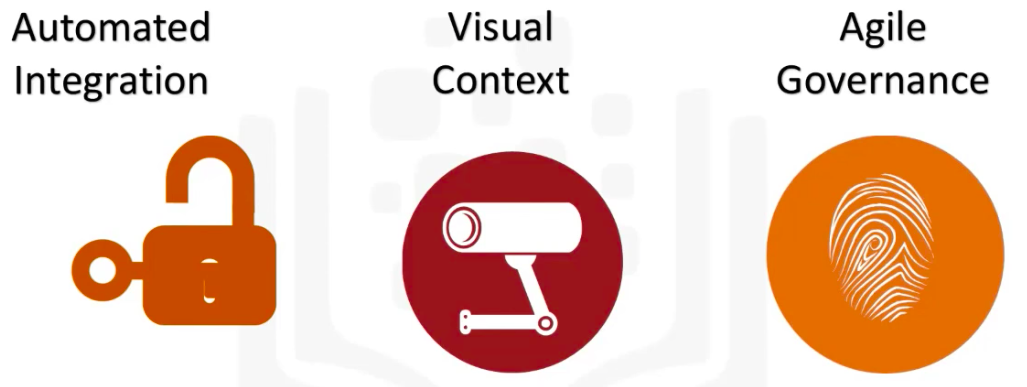
\includegraphics[scale=0.3]{img/3_Governance}
\end{figure}
\end{frame}

\begin{frame}
\frametitle{Tecnolog\'ias de la plataforma de Big Data}
\begin{figure}
\includegraphics[scale=0.3]{img/3_hadoop_vs_spark}
\end{figure}
\end{frame}

\begin{frame}
\frametitle{Big Data y Data Science}
\begin{figure}
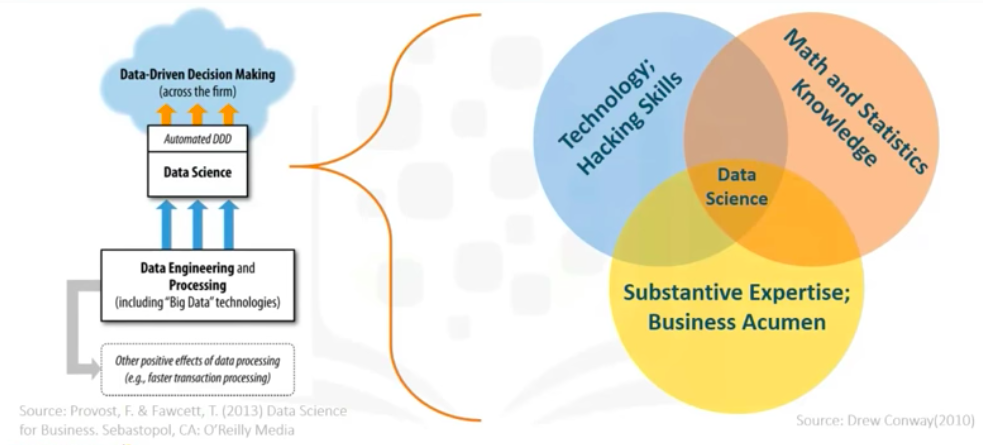
\includegraphics[scale=0.325]{img/3_BigData_DataScience}
\end{figure}
\end{frame}

\begin{frame}
\frametitle{Data Science : Proceso de destilar los datos }
\begin{figure}
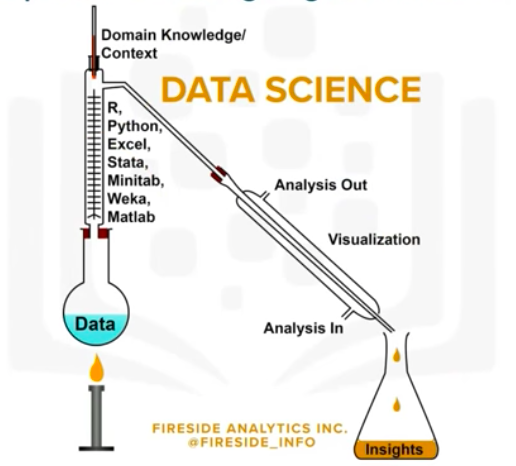
\includegraphics[scale=0.35]{img/3_DataScience_Distilling}
\end{figure}
\end{frame}

\begin{frame}
\frametitle{Data Scientist Skill }
\begin{figure}
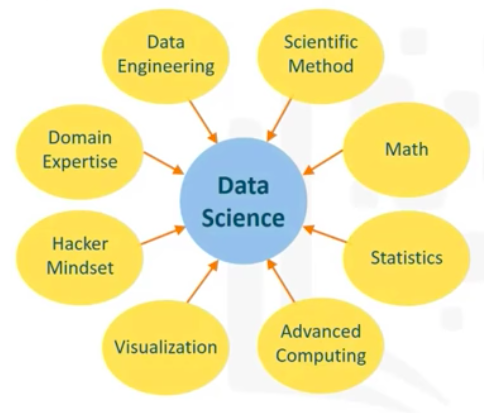
\includegraphics[scale=0.35]{img/3_DataScientist_Skill}
\end{figure}
\end{frame}

\begin{frame}
\frametitle{Modern Data Scientist }
\begin{figure}
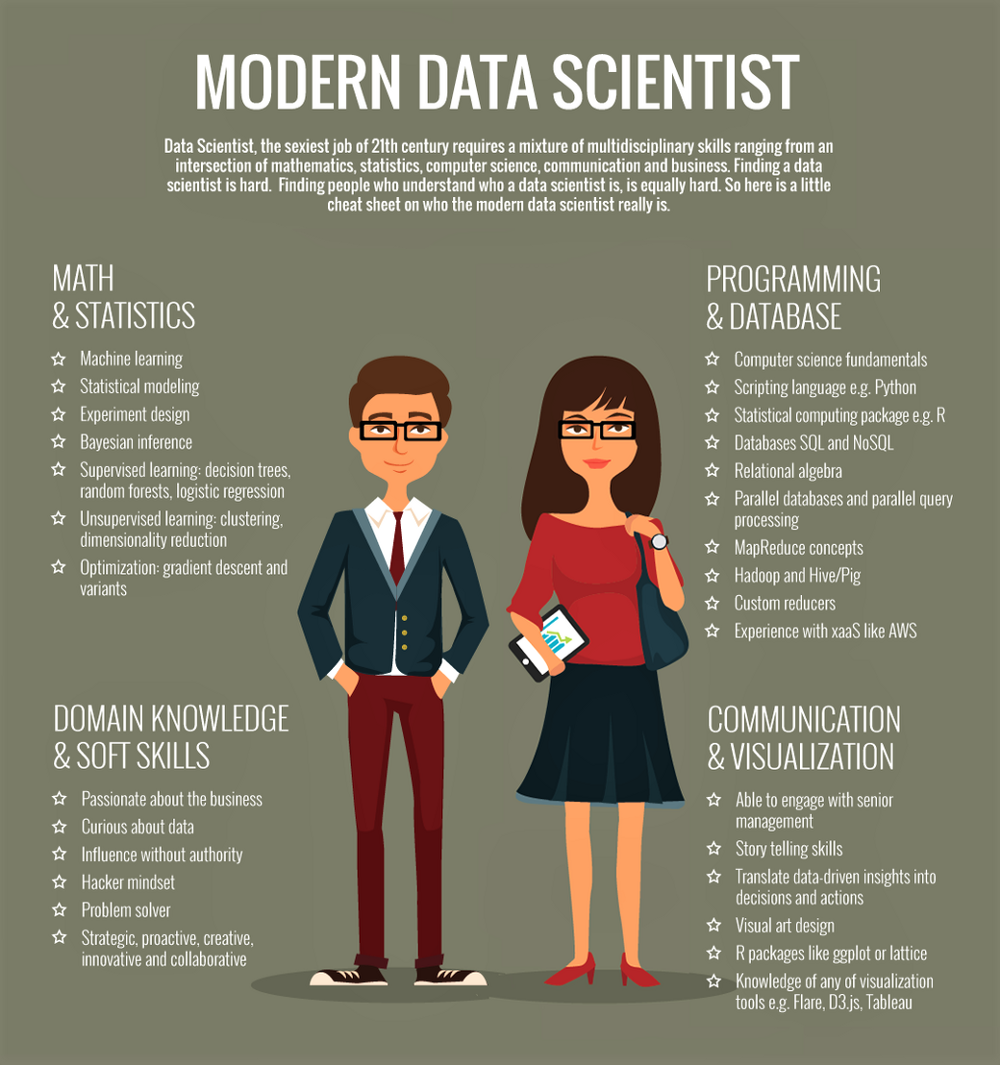
\includegraphics[scale=0.20]{img/3_DataScientist_Skill_2}
\end{figure}
\end{frame}

\begin{frame}
\frametitle{Data Science Process }
\begin{figure}
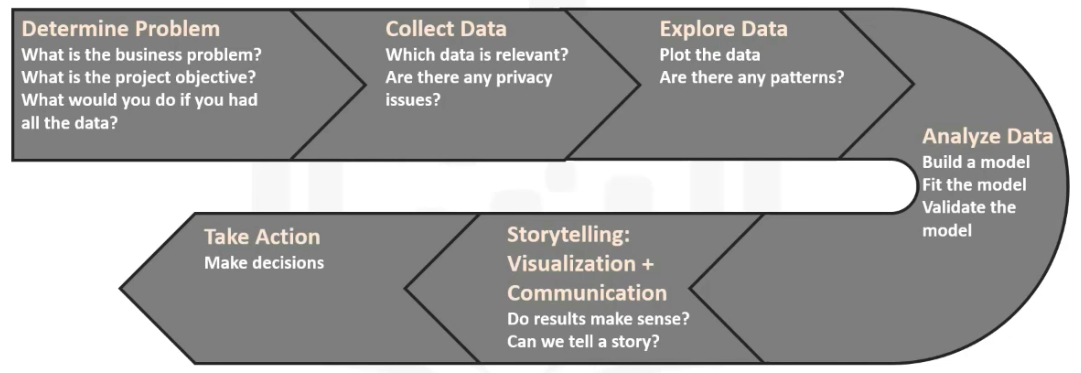
\includegraphics[scale=0.30]{img/3_DataScience_Process}
\end{figure}
\end{frame}

\begin{frame}
\frametitle{Big Data : Componentes y Ecosistemas }
\begin{figure}
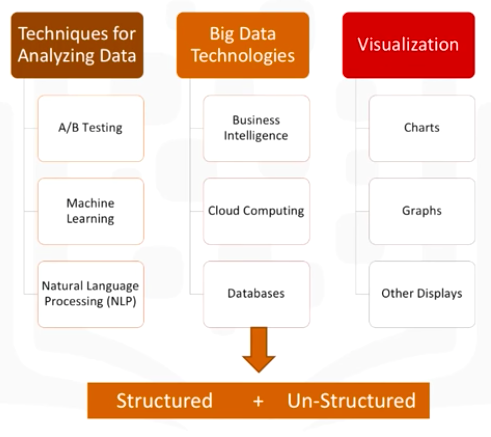
\includegraphics[scale=0.45]{img/4_BigData_Components_Ecosystems}
\end{figure}
\end{frame}





\begin{frame}
\frametitle{Conclusion}
\begin{itemize}
\item Tuple: Es una secuencia de objetos de Python inmutables. Las tuplas son secuencias, al igual que las listas.
\item List: Es un tipo de datos más versátil disponible en Python que puede escribirse como una lista de valores separados por comas (items) entre corchetes.
\item Set: Es un tipo de datos sin orden y que no permite datos repetidos
\item Dictionary: Son un tipo de estructuras de datos que permite guardar un conjunto no ordenado de pares clave-valor, siendo las claves únicas dentro de un mismo diccionario.

\end{itemize}
\end{frame}

\begin{frame}
\frametitle{Bibliography}

\begin{thebibliography}{0000}
  \bibitem{} Naomi Ceder. The Quick Python Book - Manning Publications, 2018.
\end{thebibliography}
\end{frame}



\end{document}